\section{Web-app evaluation}

This Chapter will evaluate the usability of the Agriscanner webapp using results
from a System Usability Scale (SUS) survey that was carried out via online form
in late August.

\subsection{Procedure}

Before the main section of the survey, participants were asked to consent to
standard University of Bristol privacy wording (see
Appendix~\ref{app:sus-survey}). To avoid stricter GDPR handling I did not record
identifiable information (e.g. name, email, age), which may have also encouraged
more honest responses. I also made sure to ask what device they were viewing the
project on (either mobile or desktop) as I wanted to test whether there was any
difference in usability between the two.

Participants were then asked to perform a set of four representative tasks in
the webapp. Each task involved collecting a piece of information from a
specified chart, such as finding the temperature for a particular node at a a
specified time (tasks list shown in Appendix~\ref{list-of-tasks}). Once the
tasks were completed, I asked participants to submit these answers via
multiple-choice questions.

Next, the survey presented a standard 10-question SUS, which is a Likert-scale
questionnaire commonly used to report on the usability of software systems
\cite{brookeSUS1995}. The SUS gives a score from 0 to 100, where a higher score
indicates that a system is more usable. A "good" SUS score is generally regarded
as anything above 68 \cite{sauro2016quantifying}.

Finally, there was an optional textbox for participants to fill out asking for
feedback on bugs or features they would like to see. I included this to generate
user stories for future development (Section~\ref{sec:user-story}).

By asking participants to perform the same tasks and collecting their answers, I
ensured everyone completed a valid interaction with the webapp before rating it.
This standardises the experiment context and reduces uncontrolled variance that
can arise from an open “try out my website” approach. Because I recorded the
task responses, I could also compare them to the correct answers, providing an
additional objective metric (task success) to complement the SUS.

In total, 15 participants completed the survey. Participants were recruited
mainly from friends, family and other students on my course.

\subsection{Hypotheses}

\subsubsection{Hypothesis 1}
The sample SUS score will be greater than the benchmark value of 68

\textbf{Statistic to test:} One-sample, right-tailed Wilcoxon signed-rank
test\footnote[1]{For rationale and sources on statistical testing refer to
Figure \ref{fig:appendix-note-1} in the Appendix}.

\textbf{Null and alternative hypotheses:}
\[
H_0:\ m = 68 \qquad\text{vs}\qquad H_a:\ m > 68,
\]
where \(m\) is the population median.

\subsubsection{Hypothesis 2}
The SUS scores for users on mobile will not differ significantly from those on
desktop.

\textbf{Statistic to test:} Two-sample, two-tailed Mann-Whitney U
Test\footnotemark[1].

\textbf{Null and alternative hypotheses:}
\[
H_0:\ \text{the two populations are equal} \qquad
H_a:\ \text{the two populations are not equal.}
\]

\subsection{Results}

This section summarises the key results from the survey. Refer to
Table~\ref{tab:raw-sus} in the Appendix for data per participant.

\begin{figure}[H]
    \centering
    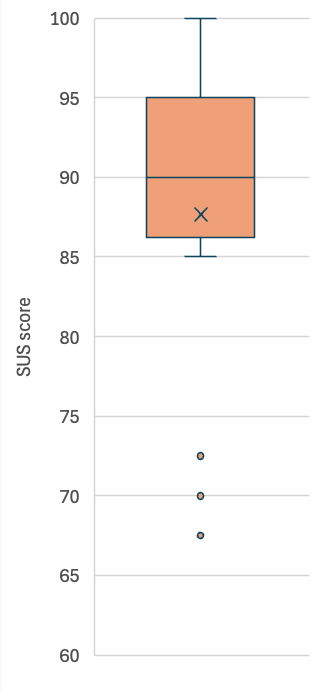
\includegraphics[width=0.3\textwidth]{contents/part-4/fig4/box-whisker.png}
    \caption{Box and whisker plot showing range of SUS scores from participants}
    \label{fig:box-whisker}
\end{figure}

\begin{table}[H]
  \centering
  \small
  \begin{minipage}[t]{0.48\textwidth}
    \centering
    \begin{tabular}{l r}
      \hline
      Metric & Value \\
      \hline
      Maximum     & 100.0 \\
      Quartile 3  & 95.0 \\
      Median      & 90.0 \\
      Mean        & 87.7 \\
      Quartile 1  & 86.3 \\
      Minimum     & 67.5 \\
      \hline
    \end{tabular}
    \captionof{table}{Summary statistics for SUS}
    \label{tab:sus-metrics}
  \end{minipage}\hfill
  \begin{minipage}[t]{0.48\textwidth}
    \centering
    \begin{tabular}{l c r}
      \hline
      Group & N & Mean SUS \\
      \hline
      Desktop & 7 & 84.3 \\
      Mobile  & 8 & 90.6 \\
      \hline
    \end{tabular}
    \captionof{table}{Mean SUS score by device}
    \label{tab:sus-by-device}
  \end{minipage}
\end{table} 

Figure~\ref{fig:box-whisker} shows a tight distribution of values between the
first and third quartiles, with most participants giving favourable ratings.
There were also a smaller number of lower ratings shown as outliers, with a
minimum score 67.5.

Table~\ref{tab:sus-metrics} shows the key metrics from the survey. The mean
score of 87.7 is well above the benchmark of 68 and indicates a high perception
of usability for the Agriscanner webapp. A one-sample Wilcoxon signed-rank test
confirmed that the median SUS score was significantly greater than 68
(\(p=0.0004\)), allowing for the rejection of the first null hypothesis \(H_0\).

Table~\ref{tab:sus-by-device} indicates that participants using mobile devices
gave slightly higher usability ratings (90.6) than those on desktop (84.3).
However, a two-sample Mann-Whitney U test revealed no statistically significant
difference between the two groups. (\(p=0.105\)). Therefore, the second null
hypothesis \(H_0\) could not be rejected at the 5\% significance level.


\begin{table}[H]
  \centering
  \begin{tabular}{r c r}
    \hline
    Question no. & Incorrect answers & Percentage incorrect\\
    \hline
    1 & 3 & 20\%\\
    2 & 1 & 7\% \\
    3 & 1 & 7\% \\
    4 & 0 & 0\% \\
    \hline
    \multicolumn{2}{r}{Overall percentage incorrect} & 8\% \\
    \hline
  \end{tabular}
  \caption{Number of incorrect answers for task quiz}
  \label{tab:correct-metrics}
\end{table}

Performance in the assigned tasks was generally good
(Table~\ref{tab:correct-metrics}), with participants answering incorrectly only
8\% of the time. Questions 2, 3 and 4 were answered correctly by almost all
participants, with only one participant failing on 2 and 3. The first question
proved the most difficult to perform accurately with 3 candidates failing. I
decided to plot the SUS score given against the percentage of correct answers
(see~\ref{app:correlation-sus}) however with an $R^2$ value of 0.0066 there was
effectively zero correlation between the two; even if there was some correlation
the small sample size and ceiling effect from so many respondents getting
perfect scores would make this difficult to detect.

\subsection{Discussion and limitations of results}

With a very high mean (87.7) and median (90) SUS score, the results here suggest
a high degree of usability. A one-sample Wilcoxon signed-rank test helps confirm
that the median score of my sample is significantly greater than the benchmark
of 68 and cannot be attributed to randomness with \(p<0.001\). This provides
quantitative evidence that the frontend development choices I have taken
(Chapter \ref{sec:front-end}) have given my webapp excellent perceived
usability. This point is further reinforced by the very high task completion
rate (92\%). The fact that users could not only perceive the system as easy to
use but could also operate it efficiently with minimal guidance validates the
chosen design approach—particularly the emphasis on a minimal, low-distraction
interface.

Additionally, the data suggest that usability on mobile devices is no different
to that on desktop devices. A two-sample Mann-Whitney U test revealed no
statistically significant difference in usability ratings between mobile and
desktop users with \(p>0.05\).

Not all the data were positive however: Two participants gave scores close to
the benchmark level of 68 and one respondent gave a score below this point. With
such a small sample it is important not to dismiss these as outliers.
Fortunately, many participants left detailed feedback on usability issues they
encountered (Figure~\ref{fig:high-sus-feedback})- including all three who gave
lower scores (Figure~\ref{fig:low-sus-feedback}). These comments provided useful
insight into specific usability issues, such as the difficulty with date
selection which directly explains the 20\% failure rate on the first task. This
qualitative feedback was then used to generate the feature requests compiled in
Table~\ref{tab:feature-requests}.

There are a number of important limitations to these findings. The sample was small
and non-random so the results are not necessarily representative of the wider
population. Because I knew many participants personally, social-desirability
bias was likely to have inflated ratings. Likewise, a high proportion of
computer-science students in the sample means these participants may have been
more familiar with web interfaces than the general public, which could also have
contributed to the higher SUS scores. While I measured the completion rate for
the user tasks I did not measure the time taken to do this. Even if users
successfully completed the tasks it may have taken a long time to do so, which
would have been a valuable metric to include here.

In conclusion, while the limitations of the sample mean the results cannot be
broadly generalised, they still provide a strong, positive indication of the
webapp's usability. An exceptionally high SUS score and a high task completion
rate demonstrate that the core design of the application succeeded in its aims.
Further, the evaluation has successfully identified specific feedback from
users, which provides a clear path to improving usability further.

\subsection{User stories from SUS survey} \label{sec:user-story}

Based on the qualitative feedback, several key themes emerged. The most
frequently mentioned issues have been summarised in
Table~\ref{tab:feature-requests} and translated into user stories to guide
future development.

\begin{table}[H]
  \centering
  \small
  \begin{tabularx}{\textwidth}{>{\RaggedRight\arraybackslash}p{0.28\textwidth}
  >{\centering\arraybackslash}p{1.5cm} >{\RaggedRight\arraybackslash}X}
    \hline
    Category & Mentions & User story \\
    \hline
    Calendar with date-range selection & 4 & As a user I want the ability to
    select date ranges so that I can quickly jump to past dates without
    repeatedly clicking through days. \\
    \hline
    Clearer way to find compare graph & 2 & As a user I want the compare graph
    to be more explicitly signposted so that I can easily find it when trying to
    compare nodes \\
    \hline
    Human readable soil moisture readings\textsuperscript{*} & 1 & As a user I
    want an option to view soil moisture in a human readable format (e.g.
    wet/dry) so that I can understand what the sensor values mean. \\
    \hline
    Tooltip granularity on chart & 1 & As a user I want smoother control when
    using the tooltip without snapping to a particular minute so that I can
    select more precise times reliably. \\
    \hline
    Way to export data  & 1 & As a user I want a way to an export weather data
    to a CSV file so that I can have offline access to it. \\
    \hline
    Switch between measurements without going back & 1 & As a user I want a
    control from within each sensor section (temperature, humidity etc) that
    allows me to switch between measurement types quickly so that I don't have
    return back to the home page between each navigation. \\
    \hline
    About page & 1 & As a user I want an "About" page describing the project and
    the data sources so that I understand the context of the data. \\
    \hline
    Specific issue with chart & 1 & As a user I want the Y axis to align with my
    screen properly so that no text is cut off and I can read the labels \\
    \hline
  \end{tabularx}
\noindent\textsuperscript{*}\small This has now been implemented on the webapp
\caption{Compiled feature requests from survey}
  \label{tab:feature-requests}
\end{table}

\subsection{General discussion on webapp}

